\documentclass{article}
\usepackage{caption}
\usepackage{subcaption}
\usepackage{graphicx}
\usepackage{tikz}
\usepackage{tikzsymbols}
\usetikzlibrary{calc}
\usepackage{float}
\usepackage{pdflscape}
\usepackage{geometry}
\geometry{a4paper, landscape, margin=1cm}
\pagestyle{empty}

\def\centerarc[#1](#2)(#3:#4:#5){\draw[#1] ($(#2)+({#5*cos(#3)},{#5*sin(#3)})$) arc (#3:#4:#5);}

\begin{document}
	\centering
	\begin{figure}[H]
			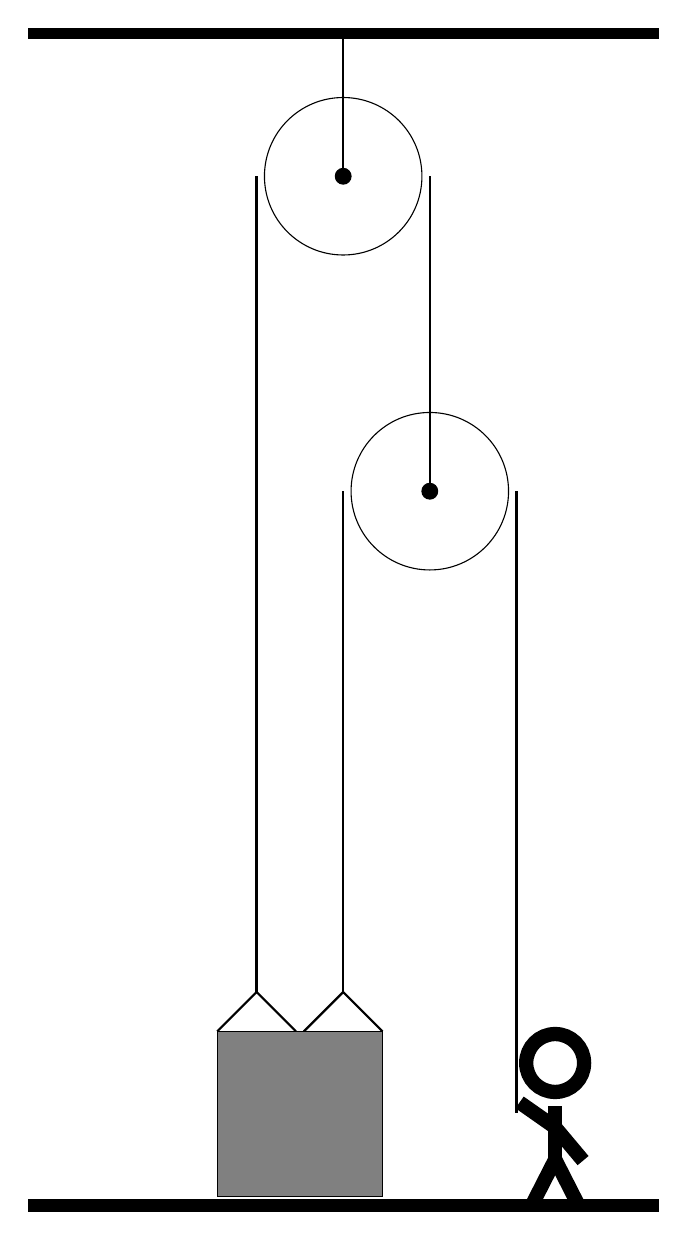
\begin{tikzpicture}
				%%%%% START %%%%%
								
				\draw[fill=black] (-2, 11.75) rectangle (6, 11.88);
				
				\draw (2, 10) circle (1);
				\draw[fill=black] (2, 10) circle (0.1);
				\draw[thick] (2, 10) -- (2, 11.75);
				
				\draw (3.1, 6) circle (1);
				\draw[fill=black] (3.1, 6) circle (0.1);
				
				\draw[thick]  (0.4, -0.86) -- (0.9, -0.36) -- (1.4, -0.86);
				\draw[thick]  (1.5, -0.86) -- (2, -0.36) -- (2.5, -0.86);
				\draw[fill=black!50] (0.4, -0.86) rectangle (2.5, -2.96);
				
				\draw[thick] (0.9, 10) -- (0.9, -0.36);
				\centerarc[thick](2, 10)(0:180:1.1);
				\draw[thick] (3.1, 10) -- (3.1, 6);
				
				\draw[thick] (2, 6) -- (2, -0.36);
				\centerarc[thick](3.1, 6)(0:180:1.1);
				\draw[thick] (4.2, 6) -- (4.2, -1.9);
				
				\node at (4.65, -2) {\Strichmaxerl[10][-35][-50]};
				
				\draw[fill=black] (-2, -3) rectangle (6, -3.15);
				%%%%% END %%%%%
			\end{tikzpicture}
	\end{figure}	
\end{document}